\documentclass[]{article}
\usepackage{lmodern}
\usepackage{amssymb,amsmath}
\usepackage{ifxetex,ifluatex}
\usepackage{fixltx2e} % provides \textsubscript
\ifnum 0\ifxetex 1\fi\ifluatex 1\fi=0 % if pdftex
  \usepackage[T1]{fontenc}
  \usepackage[utf8]{inputenc}
\else % if luatex or xelatex
  \ifxetex
    \usepackage{mathspec}
  \else
    \usepackage{fontspec}
  \fi
  \defaultfontfeatures{Ligatures=TeX,Scale=MatchLowercase}
\fi
% use upquote if available, for straight quotes in verbatim environments
\IfFileExists{upquote.sty}{\usepackage{upquote}}{}
% use microtype if available
\IfFileExists{microtype.sty}{%
\usepackage[]{microtype}
\UseMicrotypeSet[protrusion]{basicmath} % disable protrusion for tt fonts
}{}
\PassOptionsToPackage{hyphens}{url} % url is loaded by hyperref
\usepackage[unicode=true]{hyperref}
\hypersetup{
            pdftitle={Earthquake Magnitude Analysis Based on Bayesian statistics},
            pdfauthor={Zhengyu Li (10175000225); Tong Xu (1016500223)},
            pdfborder={0 0 0},
            breaklinks=true}
\urlstyle{same}  % don't use monospace font for urls
\usepackage[margin=1in]{geometry}
\usepackage{color}
\usepackage{fancyvrb}
\newcommand{\VerbBar}{|}
\newcommand{\VERB}{\Verb[commandchars=\\\{\}]}
\DefineVerbatimEnvironment{Highlighting}{Verbatim}{commandchars=\\\{\}}
% Add ',fontsize=\small' for more characters per line
\usepackage{framed}
\definecolor{shadecolor}{RGB}{248,248,248}
\newenvironment{Shaded}{\begin{snugshade}}{\end{snugshade}}
\newcommand{\KeywordTok}[1]{\textcolor[rgb]{0.13,0.29,0.53}{\textbf{#1}}}
\newcommand{\DataTypeTok}[1]{\textcolor[rgb]{0.13,0.29,0.53}{#1}}
\newcommand{\DecValTok}[1]{\textcolor[rgb]{0.00,0.00,0.81}{#1}}
\newcommand{\BaseNTok}[1]{\textcolor[rgb]{0.00,0.00,0.81}{#1}}
\newcommand{\FloatTok}[1]{\textcolor[rgb]{0.00,0.00,0.81}{#1}}
\newcommand{\ConstantTok}[1]{\textcolor[rgb]{0.00,0.00,0.00}{#1}}
\newcommand{\CharTok}[1]{\textcolor[rgb]{0.31,0.60,0.02}{#1}}
\newcommand{\SpecialCharTok}[1]{\textcolor[rgb]{0.00,0.00,0.00}{#1}}
\newcommand{\StringTok}[1]{\textcolor[rgb]{0.31,0.60,0.02}{#1}}
\newcommand{\VerbatimStringTok}[1]{\textcolor[rgb]{0.31,0.60,0.02}{#1}}
\newcommand{\SpecialStringTok}[1]{\textcolor[rgb]{0.31,0.60,0.02}{#1}}
\newcommand{\ImportTok}[1]{#1}
\newcommand{\CommentTok}[1]{\textcolor[rgb]{0.56,0.35,0.01}{\textit{#1}}}
\newcommand{\DocumentationTok}[1]{\textcolor[rgb]{0.56,0.35,0.01}{\textbf{\textit{#1}}}}
\newcommand{\AnnotationTok}[1]{\textcolor[rgb]{0.56,0.35,0.01}{\textbf{\textit{#1}}}}
\newcommand{\CommentVarTok}[1]{\textcolor[rgb]{0.56,0.35,0.01}{\textbf{\textit{#1}}}}
\newcommand{\OtherTok}[1]{\textcolor[rgb]{0.56,0.35,0.01}{#1}}
\newcommand{\FunctionTok}[1]{\textcolor[rgb]{0.00,0.00,0.00}{#1}}
\newcommand{\VariableTok}[1]{\textcolor[rgb]{0.00,0.00,0.00}{#1}}
\newcommand{\ControlFlowTok}[1]{\textcolor[rgb]{0.13,0.29,0.53}{\textbf{#1}}}
\newcommand{\OperatorTok}[1]{\textcolor[rgb]{0.81,0.36,0.00}{\textbf{#1}}}
\newcommand{\BuiltInTok}[1]{#1}
\newcommand{\ExtensionTok}[1]{#1}
\newcommand{\PreprocessorTok}[1]{\textcolor[rgb]{0.56,0.35,0.01}{\textit{#1}}}
\newcommand{\AttributeTok}[1]{\textcolor[rgb]{0.77,0.63,0.00}{#1}}
\newcommand{\RegionMarkerTok}[1]{#1}
\newcommand{\InformationTok}[1]{\textcolor[rgb]{0.56,0.35,0.01}{\textbf{\textit{#1}}}}
\newcommand{\WarningTok}[1]{\textcolor[rgb]{0.56,0.35,0.01}{\textbf{\textit{#1}}}}
\newcommand{\AlertTok}[1]{\textcolor[rgb]{0.94,0.16,0.16}{#1}}
\newcommand{\ErrorTok}[1]{\textcolor[rgb]{0.64,0.00,0.00}{\textbf{#1}}}
\newcommand{\NormalTok}[1]{#1}
\usepackage{graphicx,grffile}
\makeatletter
\def\maxwidth{\ifdim\Gin@nat@width>\linewidth\linewidth\else\Gin@nat@width\fi}
\def\maxheight{\ifdim\Gin@nat@height>\textheight\textheight\else\Gin@nat@height\fi}
\makeatother
% Scale images if necessary, so that they will not overflow the page
% margins by default, and it is still possible to overwrite the defaults
% using explicit options in \includegraphics[width, height, ...]{}
\setkeys{Gin}{width=\maxwidth,height=\maxheight,keepaspectratio}
\IfFileExists{parskip.sty}{%
\usepackage{parskip}
}{% else
\setlength{\parindent}{0pt}
\setlength{\parskip}{6pt plus 2pt minus 1pt}
}
\setlength{\emergencystretch}{3em}  % prevent overfull lines
\providecommand{\tightlist}{%
  \setlength{\itemsep}{0pt}\setlength{\parskip}{0pt}}
\setcounter{secnumdepth}{5}
% Redefines (sub)paragraphs to behave more like sections
\ifx\paragraph\undefined\else
\let\oldparagraph\paragraph
\renewcommand{\paragraph}[1]{\oldparagraph{#1}\mbox{}}
\fi
\ifx\subparagraph\undefined\else
\let\oldsubparagraph\subparagraph
\renewcommand{\subparagraph}[1]{\oldsubparagraph{#1}\mbox{}}
\fi

% set default figure placement to htbp
\makeatletter
\def\fps@figure{htbp}
\makeatother


\title{Earthquake Magnitude Analysis Based on Bayesian statistics}
\author{Zhengyu Li (10175000225) \and Tong Xu (1016500223)}
\date{2020/05/30}

\begin{document}
\maketitle

{
\setcounter{tocdepth}{2}
\tableofcontents
}
\begin{abstract}
The text of your abstract.  150 -- 250 words.This is our abstract.This is our abstract.This is our abstract.This is our abstract.This is our abstract.This is our abstract.This is our abstract.This is our abstract.This is our abstract.This is our abstract.This is our abstract.This is our abstract.This is our abstract.This is our abstract.This is our abstract.This is our abstract.This is our abstract.This is our abstract.This is our abstract.This is our abstract.This is our abstract.This is our abstract.
\end{abstract}

\section{Introduction}\label{intro}

Fiji 's urban area needs to demolish an area of old houses and then
rebuild. Because the Fiji Islands are located on the boundary between
the Pacific Plate and the Indian Plate, and are located on the Pacific
Rim Volcanic Seismic Belt, the crustal plates collide, squeeze, and
deform, making Fiji a country prone to earthquakes.Therefore, when
designing a house, the government must simultaneously consider various
factors such as budget and earthquake resistance level. Therefore, this
article will conduct a statistical analysis of the earthquakes with a
magnitude greater than 4.0 in Fiji since 1964. Find the characteristics
of the earthquake in the area and provide a reference for the local
government's architectural planning.

\section{Descriptive Statistical Analysis}\label{sec:1}

We use one of the Harvard PRIM-H project data sets(Dr.~John Woodhouse,
Dept. of Geophysics, Harvard University). The dataset has 1000
observations on the following five numeric variables:

\(x_1 = lat\) means latitude of event.

\(x_2 = long\) means longitude.

\(x_3 = depth\) means depth(km).

\(x_4 = mag\) means Richter Magnitude, which magnitudes the earthquakes.

\(x_5 = stations\) means the number of stations reporting.

Those events occurred in a cube near Fiji since 1964.

\begin{Shaded}
\begin{Highlighting}[]
\NormalTok{data <-}\StringTok{ }\NormalTok{quakes}
\NormalTok{data <-}\StringTok{ }\NormalTok{data[,}\KeywordTok{c}\NormalTok{(}\StringTok{"depth"}\NormalTok{, }\StringTok{"mag"}\NormalTok{, }\StringTok{"stations"}\NormalTok{)]}
\NormalTok{M <-}\StringTok{ }\KeywordTok{read.csv}\NormalTok{(}\StringTok{"./quakes.csv"}\NormalTok{)}
\KeywordTok{head}\NormalTok{(data)}
\end{Highlighting}
\end{Shaded}

\begin{verbatim}
##   depth mag stations
## 1   562 4.8       41
## 2   650 4.2       15
## 3    42 5.4       43
## 4   626 4.1       19
## 5   649 4.0       11
## 6   195 4.0       12
\end{verbatim}

\begin{Shaded}
\begin{Highlighting}[]
\KeywordTok{dim}\NormalTok{(data)[}\DecValTok{1}\NormalTok{]}
\end{Highlighting}
\end{Shaded}

\begin{verbatim}
## [1] 1000
\end{verbatim}

\begin{Shaded}
\begin{Highlighting}[]
\KeywordTok{summary}\NormalTok{(data)}
\end{Highlighting}
\end{Shaded}

\begin{verbatim}
##      depth            mag          stations     
##  Min.   : 40.0   Min.   :4.00   Min.   : 10.00  
##  1st Qu.: 99.0   1st Qu.:4.30   1st Qu.: 18.00  
##  Median :247.0   Median :4.60   Median : 27.00  
##  Mean   :311.4   Mean   :4.62   Mean   : 33.42  
##  3rd Qu.:543.0   3rd Qu.:4.90   3rd Qu.: 42.00  
##  Max.   :680.0   Max.   :6.40   Max.   :132.00
\end{verbatim}

\begin{Shaded}
\begin{Highlighting}[]
\KeywordTok{plot}\NormalTok{(data)}
\end{Highlighting}
\end{Shaded}

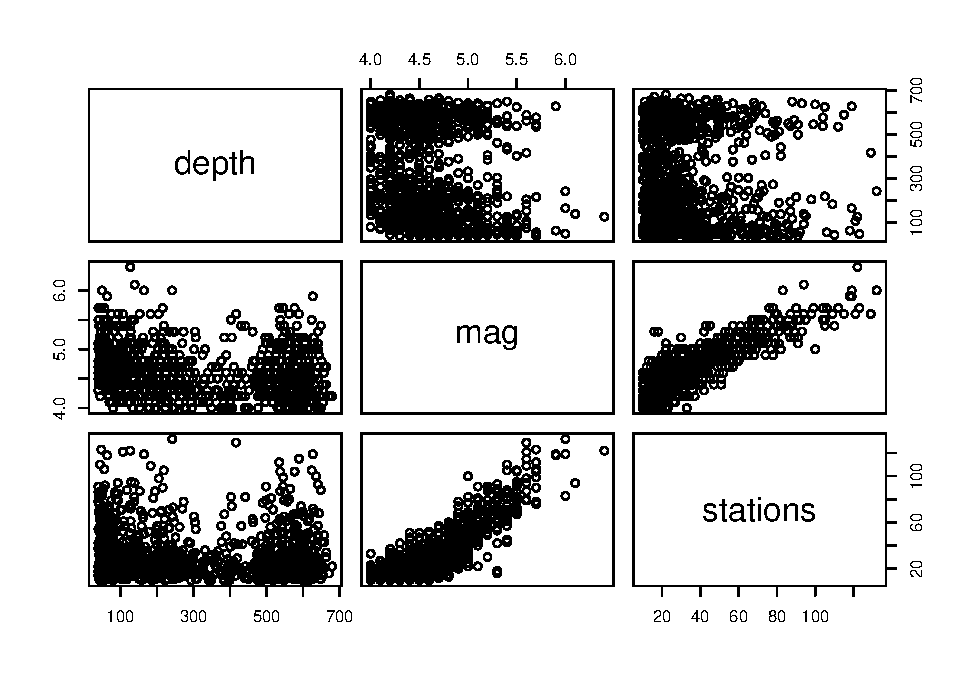
\includegraphics{Bayes-Project-by-lzy,-xt2_files/figure-latex/unnamed-chunk-1-1.pdf}

\begin{Shaded}
\begin{Highlighting}[]
\NormalTok{mag <-}\StringTok{ }\NormalTok{M}\OperatorTok{$}\NormalTok{mag}
\KeywordTok{hist}\NormalTok{(mag,}\DecValTok{15}\NormalTok{)}
\end{Highlighting}
\end{Shaded}

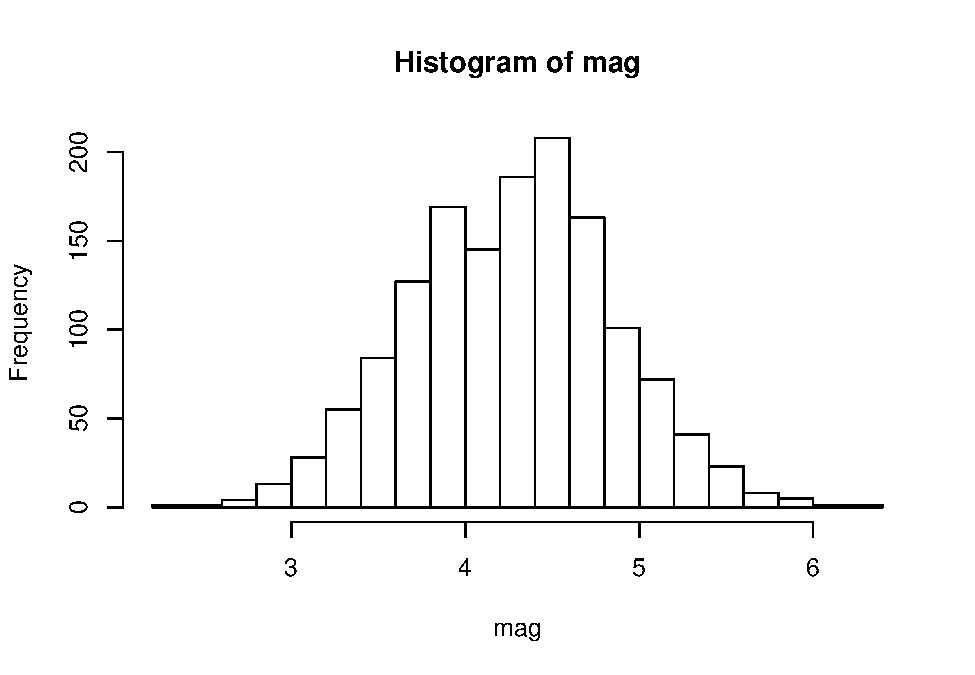
\includegraphics{Bayes-Project-by-lzy,-xt2_files/figure-latex/unnamed-chunk-1-2.pdf}

\begin{Shaded}
\begin{Highlighting}[]
\KeywordTok{par}\NormalTok{(}\DataTypeTok{mfrow =} \KeywordTok{c}\NormalTok{(}\DecValTok{1}\NormalTok{,}\DecValTok{3}\NormalTok{))}
\KeywordTok{boxplot}\NormalTok{(data}\OperatorTok{$}\NormalTok{depth, }\DataTypeTok{main  =} \StringTok{"The Boxplot of Depth(km)"}\NormalTok{);}
\KeywordTok{boxplot}\NormalTok{(data}\OperatorTok{$}\NormalTok{mag, }\DataTypeTok{main =} \StringTok{"The Boxplot of Richer Magnitude"}\NormalTok{);}
\KeywordTok{boxplot}\NormalTok{(data}\OperatorTok{$}\NormalTok{stations, }\DataTypeTok{main =} \StringTok{"The Boxplot of Stations Reporting Number"}\NormalTok{)}
\end{Highlighting}
\end{Shaded}

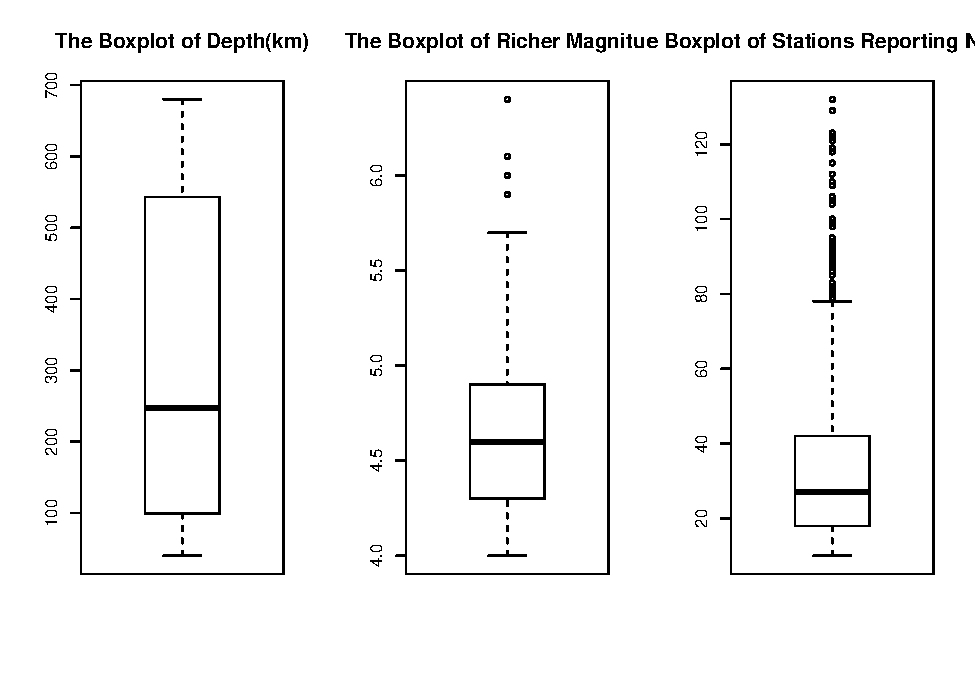
\includegraphics{Bayes-Project-by-lzy,-xt2_files/figure-latex/unnamed-chunk-1-3.pdf}

\section{Method Used in the Data
Analysis}\label{method-used-in-the-data-analysis}

\subsection{Noninformative Prior}\label{noninformative-prior}

\subsubsection{Formula Analyzing}\label{formula-analyzing}

\subsubsection{Direct Simulation}\label{direct-simulation}

\subsubsection{Indirect Simulation}\label{indirect-simulation}

\subsection{A Conjugate Joint Prior}\label{a-conjugate-joint-prior}

\section{MCMC Method}\label{mcmc-method}

\subsection{Noninformative Prior with
MCMC}\label{noninformative-prior-with-mcmc}

\subsection{Conjugate Joint Prior with
MCMC}\label{conjugate-joint-prior-with-mcmc}

\section{Hierarchical Model}\label{hierarchical-model}

\section{Results}\label{results}

\section{Conclusion}\label{conclusion}

\section{References}\label{references}

\end{document}
